%============================================================
%  MODERN B.SC / M.SC COMPUTER SCIENCE PROJECT REPORT TEMPLATE
%============================================================

\documentclass[12pt,a4paper,oneside]{report}

%------------------------------------------------------------
% PACKAGES
%------------------------------------------------------------
\usepackage[top=20mm, bottom=20mm, left=30mm, right=25mm, headheight=15pt]{geometry}
\usepackage{setspace}            % line spacing
\usepackage{lmodern}             % Modern font
\usepackage[T1]{fontenc}
\usepackage[utf8]{inputenc}
\usepackage{graphicx}
\usepackage{float}
\usepackage{booktabs}            % professional tables
\usepackage{longtable}           % multi-page tables
\usepackage{multirow}
\usepackage{array}
\usepackage{tabularx}
\usepackage{amsmath}
\usepackage{amssymb}
\usepackage{caption}
\usepackage{subcaption}
\usepackage{xcolor}
\usepackage{hyperref}
\usepackage{fancyhdr}
\usepackage{titlesec}
\usepackage{tocloft}
\usepackage{enumitem}
\usepackage{listings}
\usepackage{cite}
\usepackage{microtype}
\usepackage{colortbl}

%------------------------------------------------------------
% ===================== PROJECT DETAILS =====================
%------------------------------------------------------------
\newcommand{\ProjectTitle}{Promethee Web Application}
\newcommand{\ProjectTitleShort}{Promethee App}
\newcommand{\DegreeProgram}{Computer Science}

% Author Details
\newcommand{\StudentName}{Antonin Marouzé}
\newcommand{\StudentEmail}{antoninmarouze@gmail.com}

% Supervisor Details
\newcommand{\SupervisorName}{G. Bardis}
\newcommand{\SupervisorTitle}{Assoc. Professor} 
\newcommand{\InstitutionName}{University of West Attica}
\newcommand{\DepartmentName}{Dept. of Informatics and Computer Engineering}
\newcommand{\SubmissionYear}{2026}

% French Tutor Details
\newcommand{\FrenchTutorName}{Patricia Evraere}

%------------------------------------------------------------
% COLOURS
%------------------------------------------------------------
\definecolor{primarycolor}{RGB}{33, 150, 243} % Blue
\definecolor{tablehead}{RGB}{44, 62, 80} % Dark Blue

%------------------------------------------------------------
% LINE SPACING
%------------------------------------------------------------
\setstretch{1.05}

%------------------------------------------------------------
% WIDOW AND ORPHAN CONTROL (Empêche les lignes seules)
%------------------------------------------------------------
\clubpenalty=10000
\widowpenalty=10000
\displaywidowpenalty=10000

%------------------------------------------------------------
% CHAPTER/SECTION FORMATTING
%------------------------------------------------------------
\titleformat{\chapter}[display]
  {\normalfont\bfseries\Huge\color{tablehead}}
  {\filleft\Large\MakeUppercase{\chaptertitlename} \Huge\thechapter}
  {1ex}
  {\titlerule\vspace{1ex}\filright}
  [\vspace{1ex}\titlerule]

\titlespacing*{\chapter}{0pt}{-40pt}{10pt}

\titleformat{\section}{\bfseries\Large\color{tablehead}}{\thesection}{1em}{}
\titleformat{\subsection}{\bfseries\large\color{tablehead}}{\thesubsection}{1em}{}

%------------------------------------------------------------
% CAPTION STYLE
%------------------------------------------------------------
\captionsetup[table]{position=above, labelfont=bf, font=small}
\captionsetup[figure]{position=below, labelfont=bf, font=small}

%------------------------------------------------------------
% HEADER/FOOTER
%------------------------------------------------------------
\pagestyle{fancy}
\fancyhf{}
\fancyhead[R]{\small\textit{\ProjectTitleShort}}
\fancyhead[L]{\small\textit{\StudentName}}
\fancyfoot[C]{\thepage}
\renewcommand{\headrulewidth}{0.4pt}

%------------------------------------------------------------
% HYPERREF SETUP
%------------------------------------------------------------
\hypersetup{
  colorlinks=true,
  linkcolor=tablehead,
  citecolor=primarycolor,
  urlcolor=primarycolor,
  pdftitle={\ProjectTitle},
  pdfauthor={\StudentName}
}

%------------------------------------------------------------
% CODE LISTINGS SETUP
%------------------------------------------------------------
\lstset{
  basicstyle=\ttfamily\footnotesize,
  keywordstyle=\color{primarycolor}\bfseries,
  commentstyle=\color{gray},
  stringstyle=\color{red},
  breaklines=true,
  frame=single,
  numbers=left,
  numberstyle=\tiny\color{gray},
  backgroundcolor=\color{black!5},
  showstringspaces=false
}

%============================================================
\begin{document}
%============================================================

\pagenumbering{Roman}

%============================================================
%  TITLE PAGE
%============================================================
\begin{titlepage}
    \begin{center}
        \vspace*{0.5cm}
                
        {\Huge \bfseries \textcolor{tablehead}{\ProjectTitle}}\\[1.5cm]
        
        {\large \textit{A Project Report submitted for the degree of}}\\[0.5cm]
        {\Large \bfseries \DegreeProgram}\\[1.5cm]
        
        {\large \textit{Prepared by}}\\[0.5cm]
        {\Large \bfseries \StudentName}\\[1.5cm]
        
        {\large \textit{Under the supervision of}}\\[0.5cm]
        {\Large \bfseries \SupervisorName, \SupervisorTitle}\\[1cm]
        
        {\large \textit{Followed in France by}}\\[0.5cm]
        {\Large \bfseries \FrenchTutorName}\\[1.5cm]
        
        {\Large \bfseries \DepartmentName}\\[0.5cm]
        {\Large \bfseries \InstitutionName}\\[1cm]

        \includegraphics[width=4.5cm]{./res/picture/uni_logo.png}\\[1cm]

        {\large \SubmissionYear}
        
    \end{center}
\end{titlepage}

%============================================================
%  ABSTRACT
%============================================================
\cleardoublepage
\chapter*{Abstract}
This report details the design and implementation of a Web-based Multi-Criteria Decision Analysis (MCDA) application developed during an Erasmus+ internship at the University of West Attica. The primary goal of this project was to provide Decision Makers with a complete, interactive, and user-friendly platform to apply the PROMETHEE I and II methodologies. The application allows users to define alternatives and criteria, select from six distinct preference functions, and dynamically compute partial and complete rankings based on real-time inputs. A complementary GAIA plane visualization, computed via Principal Component Analysis, further allows Decision Makers to graphically interpret conflicting criteria and identify the best compromise alternative.

The technical solution relies on a robust three-tier architecture using Jakarta EE Servlets for the backend, Vanilla JavaScript and JSP for a responsive frontend, and PostgreSQL for persistent data storage. The entire system is containerized using Docker to ensure a reproducible deployment environment. To guarantee software reliability, comprehensive testing strategies were implemented, including unit testing for the mathematical engine, integration testing for database interactions, and end-to-end (E2E) testing for the user workflows. This project successfully bridges theoretical decision-making algorithms with modern web engineering practices, resulting in a functional decision support system.

%============================================================
%  ACKNOWLEDGEMENTS
%============================================================
\cleardoublepage
\chapter*{Acknowledgements}
I would like to express my deepest gratitude to my supervisor, Mr. Georgios Bardis, for his invaluable guidance, support, and expertise throughout this internship at the University of West Attica. 

I also extend my sincere thanks to the University of West Attica for welcoming me and providing an excellent research and development environment during this Erasmus+ mobility period. 

Finally, I am profoundly grateful to the teaching staff at the Institut Universitaire de Technologie (IUT) of Lille for the solid academic foundation in Computer Science that prepared me for this professional experience.

%============================================================
%  TABLE OF CONTENTS
%============================================================
\cleardoublepage
\tableofcontents
\cleardoublepage
\phantomsection
\addcontentsline{toc}{chapter}{List of Figures}
\listoffigures

\cleardoublepage
\phantomsection
\addcontentsline{toc}{chapter}{List of Tables}
\listoftables

%============================================================
%  MAIN CONTENT
%============================================================
\cleardoublepage
\pagenumbering{arabic}
\setcounter{page}{1}

\renewcommand{\thechapter}{\arabic{chapter}}
\renewcommand{\thesection}{\arabic{chapter}.\arabic{section}}

%------------------------------------------------------------
\chapter{Introduction}
%------------------------------------------------------------

\section{Internship Context}
I am currently completing my second year of a Bachelor Universitaire de Technologie (BUT) in Computer Science at the Institut Universitaire de Technologie (IUT) of Lille, France. As a mandatory part of this degree, representing 15 ECTS units, students are required to complete a professional internship. This mobility period within the Erasmus+ program allowed me to undertake this international experience at the University of West Attica.

\section{Mobility and Motivation}
I chose this Erasmus+ mobility to immerse myself in a new academic and professional culture, broaden my international perspective, and improve my technical English proficiency within a research and development environment.

\section{Multi-Criteria Decision Analysis (MCDA)}
Multi-Criteria Decision Analysis (MCDA) encompasses a collection of methodologies designed to evaluate and select alternatives based on multiple, often conflicting, criteria. These methods are widely employed by organizations and companies for decision support. MCDA methods aim to evaluate alternatives either in an absolute manner (providing a complete ranking) or in a relative manner (identifying strict preference, indifference, or incomparability between specific pairs). Furthermore, some methods allow for grouping alternatives into similarity groups based on shared characteristics.

\section{Project Objectives}
The primary objective of this internship, as defined in the project specification provided by the supervisor, was to design and develop a complete web application implementing both PROMETHEE I and PROMETHEE II methodologies, allowing a Decision Maker to input a performance matrix, define criteria with specific preference functions and weights, and obtain both a partial ranking (PROMETHEE I) and a complete ranking (PROMETHEE II) of the alternatives. The final deliverables include the full application source code, comprehensive documentation, and a working demonstration of the platform.

\section{Report Organization}
The first chapter of the report contains the introduction and the context of the internship. The second chapter presents the MCDA methods and the theoretical framework of the PROMETHEE algorithm, complemented by the GAIA visualization method. The third chapter outlines the functional design and use cases of the application. The fourth chapter discusses the technical architecture and implementation choices. The fifth chapter presents an extended usage example and a discussion on the application's strengths. Finally, the sixth chapter concludes the report with a synopsis of the work and future perspectives.

%------------------------------------------------------------
\chapter{MCDA Methods and Project Subject}
%------------------------------------------------------------

\section{Basics of MCDA Methods}
In the realm of MCDA, a Decision Maker (DM) expresses their preferences to evaluate a finite set of alternatives. These alternatives are judged across various attributes organized as criteria (e.g., price, area, safety rating, condition). A Decision Analyst (DA) typically guides the DM through this process, organizing information and applying mathematical models. 

MCDA is broadly divided into two main schools of thought:
\begin{itemize}
    \item \textbf{Utility Function Methods (American School):} Represented by weighted sum methodologies and the Analytic Hierarchy Process (AHP).
    \item \textbf{Outranking Methods (European School):} Focused on pairwise comparisons, with main representatives being ELECTRE and PROMETHEE.
\end{itemize}
These two families cover the vast majority of MCDA applications encountered in practice~\cite{belton2002}.

\section{Implemented Method: PROMETHEE Algorithm}
The PROMETHEE method (Preference Ranking Organization Method for Enrichment of Evaluations) was introduced by Brans and Vincke~\cite{brans1985} and is based on the principle of pairwise comparisons.

\subsection{Unicriterion Preference}
For a criterion $j$, we calculate the difference between the evaluation of alternative $a$ and alternative $b$:
\begin{equation}
    d_j(a, b) = g_j(a) - g_j(b)
\end{equation}
This difference is transformed into a preference degree $P_j(a,b) \in [0, 1]$ using one of the six standard preference functions:
\begin{enumerate}
    \item \textbf{Type 1 (Usual):} $P(d) = 1$ if $d > 0$, else $0$.
    \item \textbf{Type 2 (U-Shape):} $P(d) = 1$ if $d > q$, else $0$ (uses indifference threshold $q$).
    \item \textbf{Type 3 (V-Shape):} $P(d) = d/p$ if $0 < d \le p$, and $1$ if $d > p$ (uses preference threshold $p$).
    \item \textbf{Type 4 (Level):} $P(d) = 0.5$ if $q < d \le p$, and $1$ if $d > p$.
    \item \textbf{Type 5 (V-Shape Indiff.):} $P(d) = (d-q)/(p-q)$ if $q < d \le p$, and $1$ if $d > p$.
    \item \textbf{Type 6 (Gaussian):} $P(d) = 1 - e^{-d^2/2s^2}$ (uses standard deviation $s$).
\end{enumerate}

\subsection{Global Preference and Flows}
The aggregated preference index $\pi(a,b)$ is calculated using criterion weights $w_j$:
\begin{equation}
    \pi(a, b) = \sum_{j=1}^{k} w_j P_j(a, b)
\end{equation}
where the weights $w_j$ are normalized such that $\sum_{j=1}^{k} w_j = 1$ and $w_j \geq 0$.

PROMETHEE I calculates the positive flow $\Phi^+(a)$ (dominance power) and the negative flow $\Phi^-(a)$ (weakness):
\begin{equation}
    \Phi^+(a) = \frac{1}{n-1} \sum_{x \neq a} \pi(a, x) \quad , \quad \Phi^-(a) = \frac{1}{n-1} \sum_{x \neq a} \pi(x, a)
\end{equation}

\subsection{PROMETHEE I vs PROMETHEE II}
\textbf{PROMETHEE I} establishes a partial ranking. Alternative $a$ is preferred to $b$ ($a P^I b$) if $\Phi^+(a) \ge \Phi^+(b)$ and $\Phi^-(a) \le \Phi^-(b)$, with at least one strict inequality. If $\Phi^+(a) > \Phi^+(b)$ and $\Phi^-(a) > \Phi^-(b)$ (or vice-versa), the alternatives are considered \textbf{incomparable}. Two alternatives $a$ and $b$ are considered \textbf{indifferent} ($a I^I b$) if $\Phi^+(a) = \Phi^+(b)$ and $\Phi^-(a) = \Phi^-(b)$.

\textbf{PROMETHEE II} establishes a complete ranking by calculating the \textbf{Net Flow}:
\begin{equation}
    \Phi(a) = \Phi^+(a) - \Phi^-(a)
\end{equation}
The alternative with the highest net flow is ranked first.

\subsection{GAIA Plane Visualization}
The GAIA (Geometrical Analysis for Interactive Aid) plane~\cite{mareschal2013} provides a powerful 2D visualization complementing the PROMETHEE rankings. It is obtained by applying a \textbf{Principal Component Analysis (PCA)} to the matrix of unicriterion net flows $\phi_j(a)$, defined as:
\begin{equation}
    \phi_j(a) = \frac{1}{n-1} \sum_{x \neq a} \left[ P_j(a, x) - P_j(x, a) \right]
\end{equation}
This produces an $N \times C$ matrix (alternatives $\times$ criteria), which is then projected onto the first two principal components. On the resulting plane:
\begin{itemize}
    \item \textbf{Alternatives} are represented as points. Nearby points indicate similar performance profiles.
    \item \textbf{Criteria} are represented as vectors (arrows) from the origin. An alternative located in the direction of a criterion vector performs well on that criterion.
    \item \textbf{Criteria agreement:} Two vectors pointing in the same direction indicate correlated criteria; opposite vectors indicate conflicting criteria.
    \item \textbf{The decision axis $\pi$} (a weighted combination of all criterion vectors) points toward the best compromise according to the assigned weights.
\end{itemize}
The percentage of \textbf{variance explained} indicates the quality of the 2D projection: a value above 70--80\% means the plane faithfully represents the decision problem.

%------------------------------------------------------------
\chapter{Functional Design}
%------------------------------------------------------------

\section{User Interface and Features}
The application provides a dynamic web interface allowing users to define decision problems without technical expertise. The development process started with the design of an initial wireframe mockup (Figure~\ref{fig:ui_mockup}) to establish the core user experience before implementation. The layout is divided into a data entry matrix, a pairwise comparison tool, and a final results table. The final implemented interface is shown in Figure~\ref{fig:ui_matrix}.

\begin{figure}[H]
  \centering
  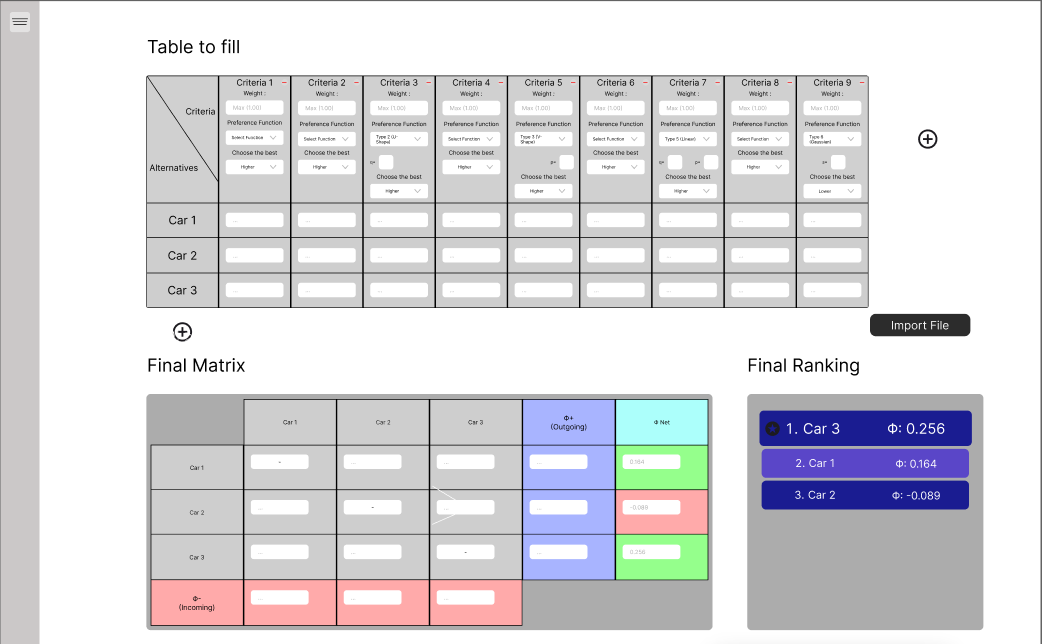
\includegraphics[width=0.95\textwidth]{./res/application_picture/Model_app.png}
  \caption{Initial Wireframe Mockup: Early design of the application's layout and data entry matrix.}
  \label{fig:ui_mockup}
\end{figure}

\begin{figure}[H]
  \centering
  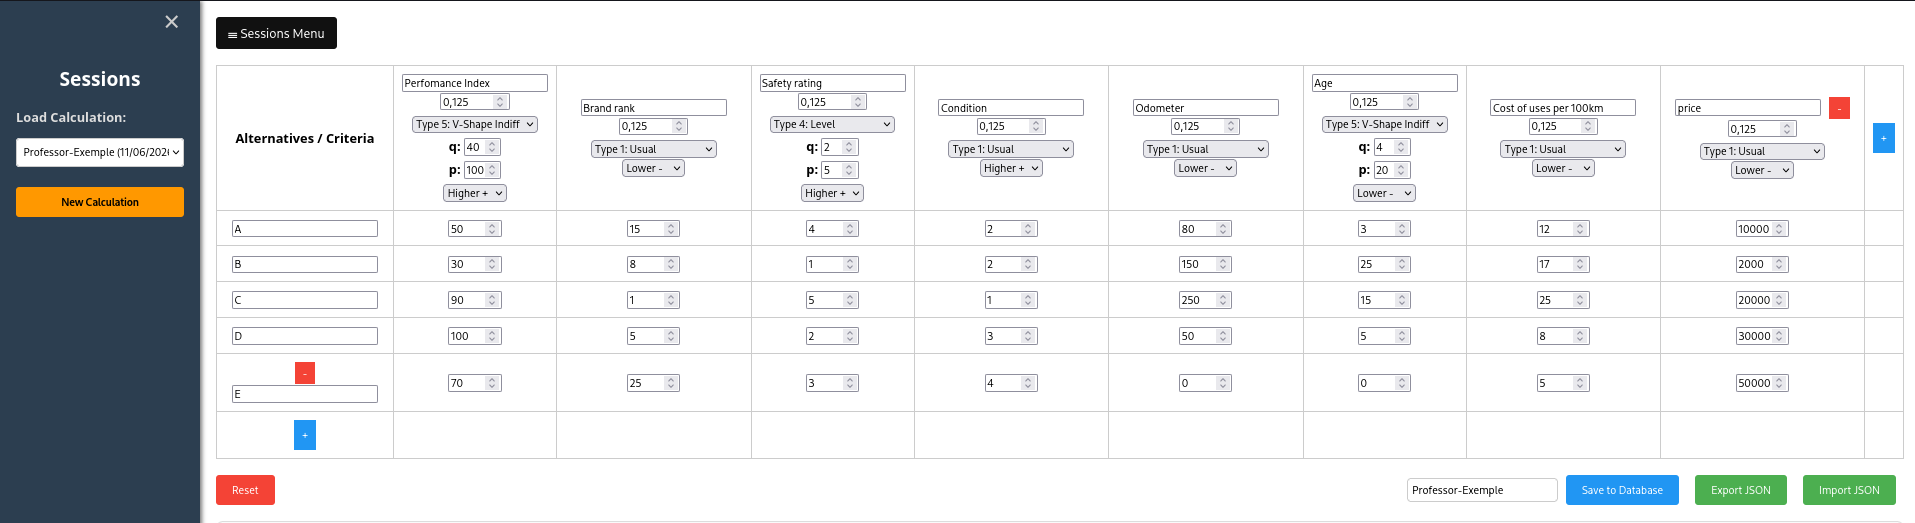
\includegraphics[width=0.95\textwidth]{./res/application_picture/Matrix_alternative_criteria.png}
  \caption{Final Data Entry Interface: Users can dynamically add criteria and alternatives, choosing weights and preference functions through simple dropdowns and inputs.}
  \label{fig:ui_matrix}
\end{figure}

Key functionalities include:
\begin{itemize}
    \item \textbf{Dynamic Matrix:} Real-time addition/removal of criteria and alternatives.
    \item \textbf{Real-time Calculation:} The results update automatically as soon as the criterion weights sum to 1.0.
    \item \textbf{Pairwise Analysis:} A dedicated section to compare any two alternatives criterion-by-criterion.
    \item \textbf{GAIA Visualization:} An interactive 2D scatter plot allowing the Decision Maker to visually interpret conflicting criteria and identify the best compromise alternative.
\end{itemize}

The interface is designed to support both roles identified in MCDA methodology: the \textbf{Decision Maker (DM)}, who inputs evaluations and interprets results, and the \textbf{Decision Analyst (DA)}, who configures the criteria, weights, and preference functions.

\section{Usage Scenario and Use Cases}
Consider a Decision Maker wishing to select a company vehicle. They open the application and create a new session named ``Vehicle Purchase 2026''. They add three alternatives (Car A, Car B, Car C) and define three criteria: Price (to minimize), Quality (to maximize), and Delivery Time (to minimize). For each criterion, they select an appropriate preference function and assign weights summing to 1.0. As they fill in the evaluation scores, the PROMETHEE II ranking updates in real time. Finally, they use the pairwise comparison tool to analyze why Car A ranks above Car C on specific criteria, and save the session for future reference.

The full set of user interactions and functionalities described in this scenario are formalized in the Use Case diagram below (see Figure \ref{fig:usecase}).

\begin{figure}[H]
  \centering
  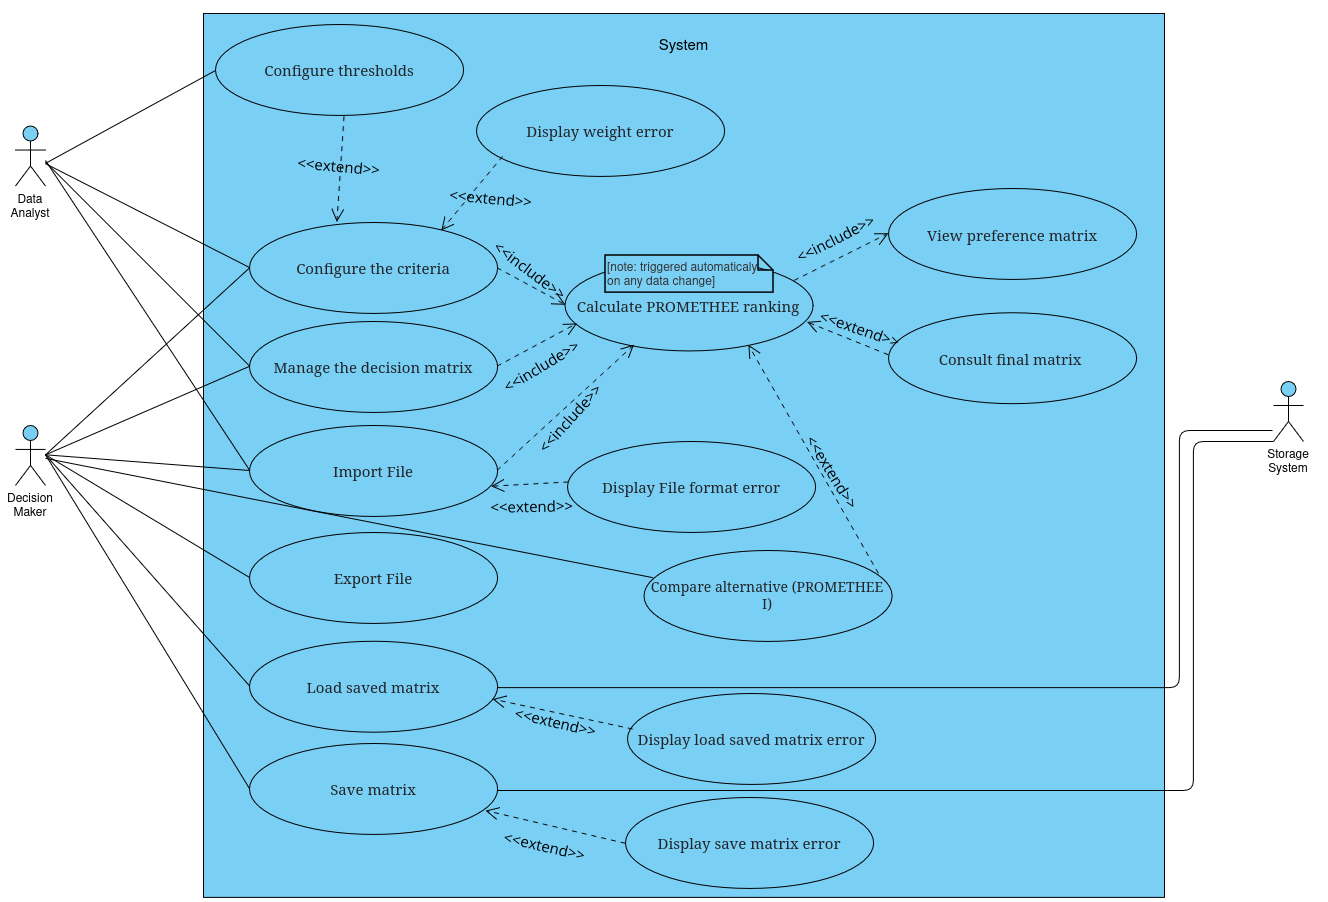
\includegraphics[width=0.85\textwidth]{./res/Uml/Use_Case_Diagram.png}
  \caption{Use Case Diagram: Illustrates the primary interactions a user has with the system, such as managing the matrix and exporting results.}
  \label{fig:usecase}
\end{figure}

\section{Data Storage Overview}
The application stores four types of information to ensure data persistence: \textbf{Sessions} (the global decision problem), \textbf{Criteria} (weights and preference function parameters), \textbf{Alternatives} (names and identities), and \textbf{Evaluations} (the raw performance scores linking each alternative to each criterion). The detailed relational schema is presented in the Technical Design chapter.


\section{Requirements Traceability}
Table~\ref{tab:traceability} maps each requirement from the official project specification to its corresponding implementation.

\begin{table}[H]
\caption{Requirements Traceability Matrix}
\label{tab:traceability}
\centering
\begin{tabular}{p{5cm}p{7cm}c}
\toprule
\textbf{Requirement} & \textbf{Implementation} & \textbf{Status} \\
\midrule
Enter alternatives and characteristics & Dynamic matrix interface (Sec 3.1) & Done \\
Define criteria with parameters & Criterion configuration with 6 preference functions & Done \\
Visually interactive result updates & Real-time AJAX recalculation & Done \\
Modify alternatives/parameters dynamically & Live matrix editing & Done \\
\bottomrule
\end{tabular}
\end{table}

%------------------------------------------------------------
\chapter{Technical Design}
%------------------------------------------------------------

\section{Implementation Choices and Technologies}
The backend is implemented using \textbf{Jakarta EE Servlets}~\cite{jakartaee}, chosen for its robustness and my strong academic familiarity with the Java ecosystem. \textbf{Apache Tomcat 10.1}~\cite{TomcatDoc} was selected for its open-source nature and widespread industry adoption as a stable Servlet container. For data persistence, \textbf{PostgreSQL}~\cite{PostgreSQLDoc} was preferred over alternatives for its strict ACID compliance and advanced support for relational data. Database connectivity is ensured via the \textbf{PostgreSQL JDBC Driver}, which enables the Jakarta EE application to communicate with the database using standard SQL queries. Finally, \textbf{Docker}~\cite{DockerDoc} was employed to ensure a fully reproducible deployment environment across different machines.

The frontend uses vanilla JavaScript and JavaServer Pages (JSP) to maintain high performance and avoid the overhead of heavy frontend frameworks, while still leveraging lightweight, focused libraries such as \textbf{Chart.js} (loaded via CDN) for specific visualization needs such as the interactive GAIA plane. To improve the user experience, the application utilizes the browser's \textbf{localStorage} to automatically cache the matrix state during editing.

\section{System Architecture and Deployment}
The application follows a classic three-tier architecture, physically distributed across multiple nodes. As detailed in the Deployment Diagram (see Figure \ref{fig:deployment}), the system consists of a client browser, an application server container, and a database container.

The two API endpoints are strictly separated by responsibility: 
\begin{itemize}
    \item \texttt{PrometheeServlet} (\texttt{/calculate}) is stateless and processes raw JSON matrix data to return computed flows.
    \item \texttt{SessionServlet} (\texttt{/api/sessions}) manages stateful CRUD operations against the PostgreSQL database.
\end{itemize}

The entire stack is orchestrated using Docker Compose, which seamlessly networks the Tomcat application container with the database container, mounting a local volume for persistent storage and initializing the schema automatically.

\begin{figure}[H]
  \centering
  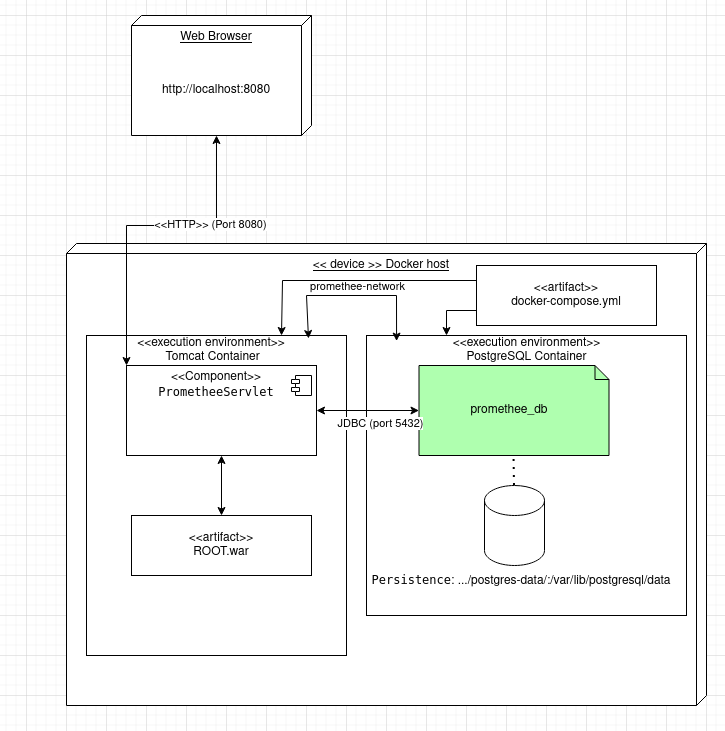
\includegraphics[width=0.85\textwidth]{./res/Uml/Deployment_Diagram.png}
  \caption{Deployment Diagram: Shows the physical distribution of the system components.}
  \label{fig:deployment}
\end{figure}

\section{Logical Data Model (MLD)}
The relational structure of the database, illustrated in Figure~\ref{fig:mld}, was designed to support the PROMETHEE data model, ensuring a clear separation between session metadata, criteria parameters, and raw evaluation scores.
\begin{figure}[H]
  \centering
  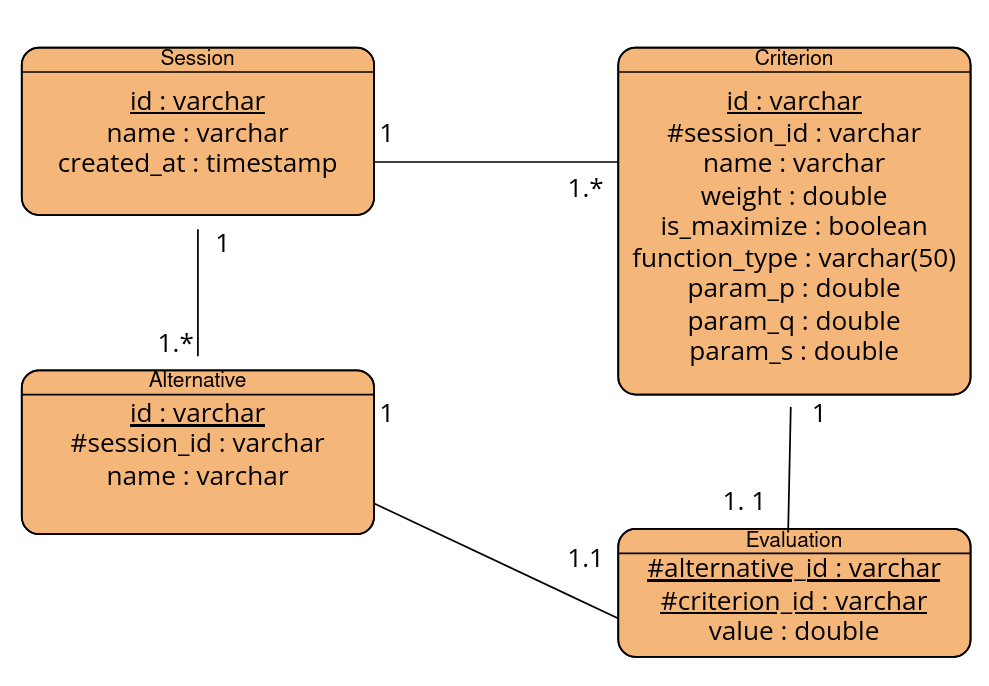
\includegraphics[width=0.85\textwidth]{./res/Uml/MLD_Database.png}
  \caption{Logical Data Model: Relational schema including primary and foreign key associations.}
  \label{fig:mld}
\end{figure}

\section{MVC and Service Layer Architecture}
To ensure maintainability and scalability, the code follows a strict Model-View-Controller (MVC) pattern, enhanced with a dedicated Service layer to decouple concerns.
\begin{itemize}
    \item \textbf{Controller:} Managed by Jakarta EE Servlets (\texttt{PrometheeServlet} and \allowbreak \texttt{SessionServlet}), which handle incoming HTTP requests and delegate logic to the service layer.
    \item \textbf{Service:} The \texttt{PrometheeService} centralizes the business logic, including JSON data parsing (utilizing the powerful \textbf{Jackson}~\cite{jackson} library) and the orchestration of the mathematical calculation engine. It also implements the \textbf{DTO (Data Transfer Object)} pattern via the \texttt{CalculationResult} class to efficiently package API responses.
    \item \textbf{Model:} Classes (\texttt{Alternative}, \allowbreak \texttt{Criterion}, \allowbreak and \allowbreak \texttt{Session}) encapsulate the PROMETHEE data structures and mathematical rules.
    \item \textbf{DAO:} The \texttt{SessionDAO} handles interaction with the PostgreSQL database using standard JDBC.
    \item \textbf{View:} The presentation layer is centralized in the \texttt{index.jsp} file, which provides the responsive visual structure and dynamically interacts with the controllers via asynchronous JavaScript (AJAX) calls.
\end{itemize}

The complete object-oriented structure is illustrated in Figure~\ref{fig:classdiagram}, while Figure~\ref{fig:sequence} details the execution flow of a calculation request from the client browser through the MVC layers to the mathematical engine.

\begin{figure}[H]
  \centering
  
\includegraphics[width=0.85\textwidth]{./res/Uml/Diagram_Class.png}
  \caption{Class Diagram: Internal object-oriented structure of the mathematical model.}
  \label{fig:classdiagram}
\end{figure}

\begin{figure}[H]
  \centering
  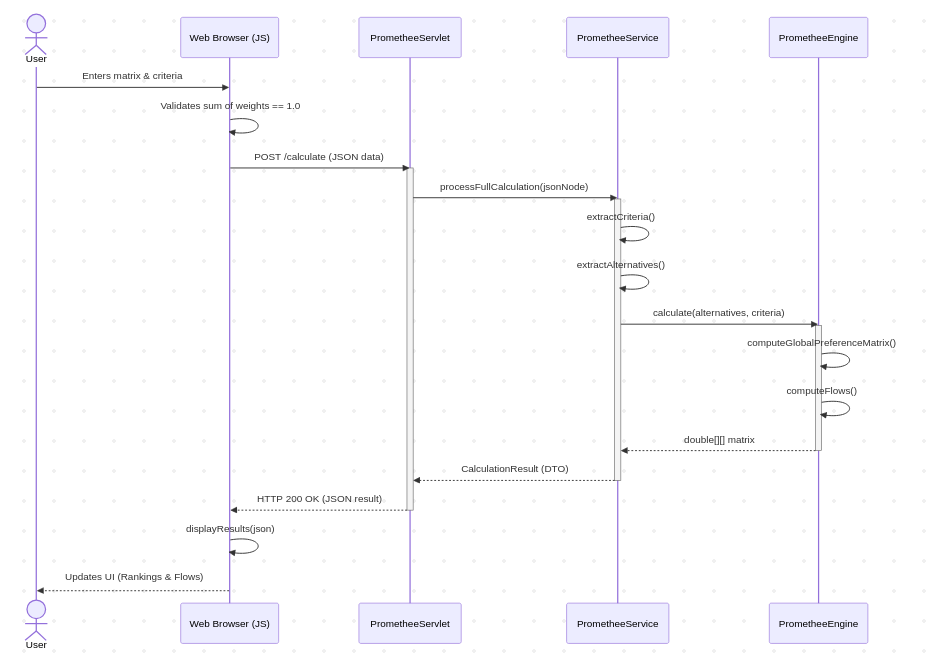
\includegraphics[width=0.95\textwidth]{./res/Uml/Sequence_Diagram.png}
  \caption{Sequence Diagram: Complete execution flow of a calculation request from the client browser through the MVC layers to the mathematical engine.}
  \label{fig:sequence}
\end{figure}

\section{Algorithmic Engine Implementation}
The core calculation engine (\texttt{PrometheeEngine}) is strictly decoupled from the web layer. It operates directly on the \texttt{Alternative} and \texttt{Criterion} objects. The following code snippet illustrates the calculation of the positive and negative outranking flows, demonstrating the $\mathcal{O}(N^2)$ algorithmic complexity resulting from the nested loop across all alternatives.

\begin{lstlisting}[language=Java, caption={Calculation of Outranking Flows}, label={lst:flows}]
public void computeFlows(List<Alternative> alternatives, double[][] matrix) {
    int n = alternatives.size();
    for (int i = 0; i < n; i++) {
        double phiPlus = 0;
        double phiMinus = 0;
        for (int j = 0; j < n; j++) {
            if (i == j) continue;
            phiPlus += matrix[i][j];
            phiMinus += matrix[j][i];
        }
        Alternative a = alternatives.get(i);
        a.setPhiPlus(phiPlus / (n - 1));
        a.setPhiMinus(phiMinus / (n - 1));
        a.setPhiNet(a.getPhiPlus() - a.getPhiMinus());
    }
}
\end{lstlisting}

\subsection{GAIA Engine Implementation}
A dedicated \texttt{GaiaEngine} class implements the PCA computation for the GAIA plane without any external mathematical library. The algorithm performs the following steps:
\begin{enumerate}
    \item Builds the unicriterion net flow matrix ($N \times C$) from the raw evaluations.
    \item Centers the matrix by subtracting column means.
    \item Computes the covariance matrix ($C \times C$).
    \item Extracts the two dominant eigenvectors using the \textbf{Power Iteration} method.
    \item Projects alternatives (as points) and criteria (as vectors) onto the 2D plane.
    \item Computes the \textbf{decision axis $\pi$} as the weighted projection of criterion vectors.
\end{enumerate}
The projected coordinates are serialized as JSON and sent to the frontend, where they are rendered as an interactive scatter plot using the \textbf{Chart.js} library loaded via CDN.

\section{Testing and Quality Assurance}
To ensure the reliability and correctness of the application, a comprehensive testing strategy was implemented within the \texttt{src/test} directory. 
\begin{itemize}
    \item \textbf{Unit Testing:} The core mathematical engine (\texttt{PrometheeEngine} and preference functions) is heavily tested to guarantee that the PROMETHEE flows and calculations are strictly accurate.
    \item \textbf{Integration Testing:} The Data Access Object (DAO) layer and the PostgreSQL database connectivity are validated through integration tests to ensure data persistence and retrieval function correctly.
    \item \textbf{End-to-End (E2E) Testing:} The complete user workflows, from creating a matrix in the frontend to calculating the results via the backend API, are verified through E2E tests simulating real user interactions.
\end{itemize}
This rigorous approach guarantees the robustness of the decision-making platform in a production-like environment.

\section{Security Considerations}
All database interactions within \texttt{SessionDAO} use \texttt{PreparedStatement} objects rather than concatenated SQL strings. This approach ensures that variables are safely bound, completely eliminating SQL injection vulnerabilities.

\begin{lstlisting}[language=Java, caption={Using PreparedStatement to prevent SQL Injection}, label={lst:prepstatement}]
try (PreparedStatement pstmt = conn.prepareStatement(insertSessionSql)) {
    pstmt.setString(1, session.getId());
    pstmt.setString(2, session.getName());
    pstmt.setTimestamp(3, session.getCreatedAt());
    pstmt.executeUpdate();
}
\end{lstlisting}

Additionally, input validation is performed at the Service layer before any data reaches the persistence layer, ensuring that malformed JSON payloads cannot compromise the database state. 

Furthermore, to prevent Insecure Direct Object Reference (IDOR) vulnerabilities, primary keys across all entities are generated in Java using Universally Unique Identifiers (UUIDs), rather than predictable auto-incrementing integers. This ensures that malicious users cannot easily guess or enumerate resource identifiers to access unauthorized data.

\begin{lstlisting}[language=Java, caption={UUID Generation for Primary Keys}, label={lst:uuid}]
this.id = UUID.randomUUID().toString();
\end{lstlisting}
%------------------------------------------------------------
\chapter{Discussion}
%------------------------------------------------------------

\section{Extended Experiment and Usage Example}
To validate the application, a vehicle selection scenario was implemented. Three alternatives were compared against three criteria using the parameters defined in Table \ref{tab:exp_input}.

\begin{table}[H]
\caption{Experiment Data: Input Matrix and Parameters}
\label{tab:exp_input}
\centering
\begin{tabular}{lccc}
\toprule
\textbf{Alternative} & \textbf{Price (Min, V-Shape)} & \textbf{Quality (Max, Usual)} & \textbf{Delay (Min, U-Shape)} \\
\textbf{Weight} & \textbf{w=0.5, p=10} & \textbf{w=0.3} & \textbf{w=0.2, q=5} \\
\midrule
Car A & 80 & 10 & 15 \\
Car B & 90 & 9 & 12 \\
Car C & 75 & 8 & 20 \\
\bottomrule
\end{tabular}
\end{table}

The application generated the following PROMETHEE II results, illustrated in Figure~\ref{fig:ui_results_p2} and summarized in Table~\ref{tab:exp_results}:

\begin{table}[H]
\caption{Experiment Results: Calculated Flows}
\label{tab:exp_results}
\centering
\begin{tabular}{lcccc}
\toprule
\textbf{Alternative} & \textbf{$\Phi^+$ (Power)} & \textbf{$\Phi^-$ (Weakness)} & \textbf{$\Phi$ (Net Flow)} & \textbf{Rank} \\
\midrule
Car A & 0.5500 & 0.1250 & 0.4250 & 1 \\
Car C & 0.3750 & 0.4000 & -0.0250 & 2 \\
Car B & 0.2500 & 0.6500 & -0.4000 & 3 \\
\bottomrule
\end{tabular}
\end{table}

\begin{figure}[H]
  \centering
  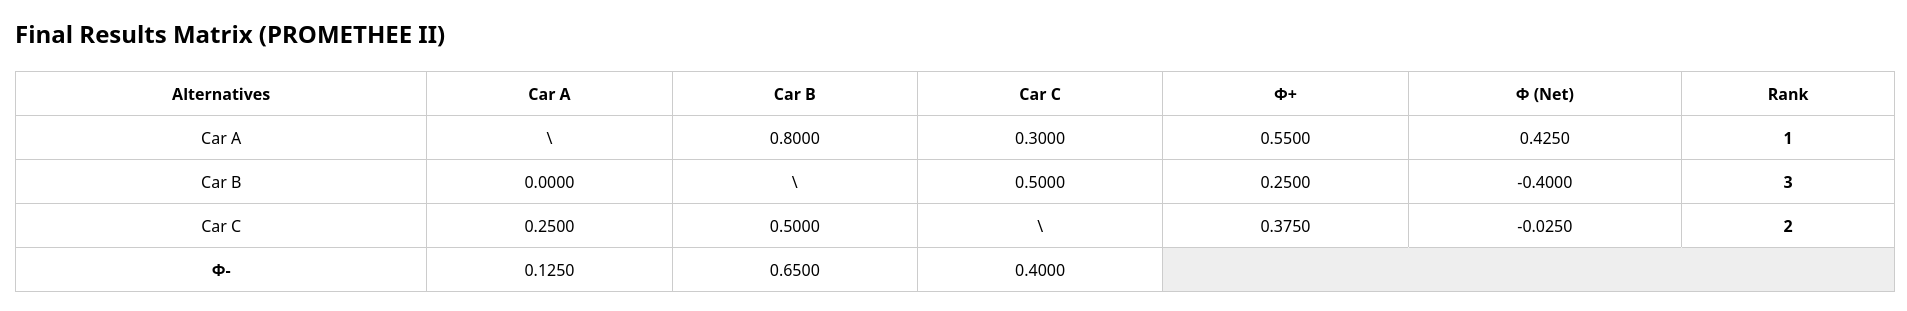
\includegraphics[width=0.95\textwidth]{./res/application_picture/Promethee_II_Matrix.png}
  \caption{Results Interface: PROMETHEE II complete ranking with positive, negative, and net flows.}
  \label{fig:ui_results_p2}
\end{figure}

Figure~\ref{fig:ui_results_p1} shows the corresponding PROMETHEE I global relation matrix used for pairwise comparison.

\begin{figure}[H]
  \centering
  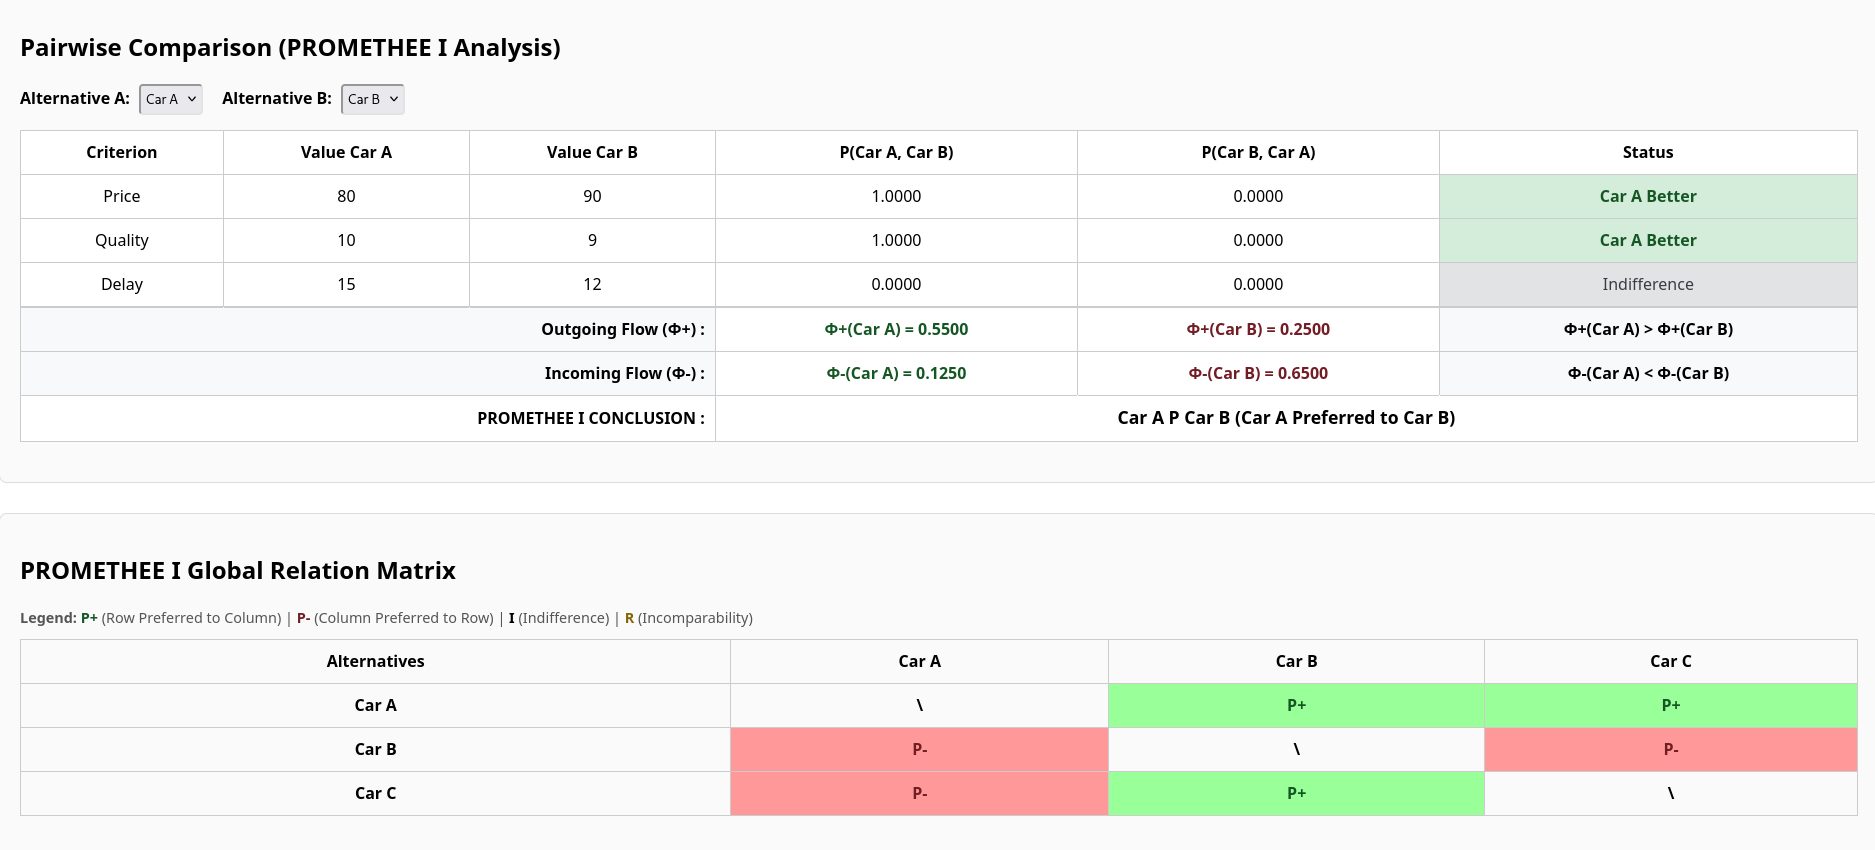
\includegraphics[width=0.95\textwidth]{./res/application_picture/Promethee_I_picture.png}
  \caption{Results Interface: PROMETHEE I global relation matrix and pairwise comparison.}
  \label{fig:ui_results_p1}
\end{figure}

The results confirm that Car A is the best overall choice, driven primarily by its competitive price (dominant criterion with w=0.5). Car C ranks second despite its lower price because its significantly longer delivery time (20 days vs 15 for Car A) penalizes it on that criterion. Car B ranks last due to its highest price (90), which is decisively penalized by the V-Shape function with p=10.

Applying PROMETHEE I, Car A and Car C are comparable ($\Phi^+(A) > \Phi^+(C)$ and $\Phi^-(A) < \Phi^-(C)$), confirming Car A's dominance. However, Car A and Car B are also comparable, while Car B and Car C present an interesting case worth examining in the pairwise tool.

The GAIA plane (Figure~\ref{fig:gaia_plane}) provides a complementary visual interpretation of these results. On the plane, Car A is positioned closest to the decision axis $\pi$, confirming it as the best overall compromise. The Price criterion vector and the Delay criterion vector point in divergent directions, visually illustrating the trade-off between cost and delivery time that the Decision Maker must navigate. For this experiment, the projection explains \textbf{100.0\%} of the total variance, confirming that the 2D plane provides a faithful representation of the decision problem.

\begin{figure}[H]
  \centering
  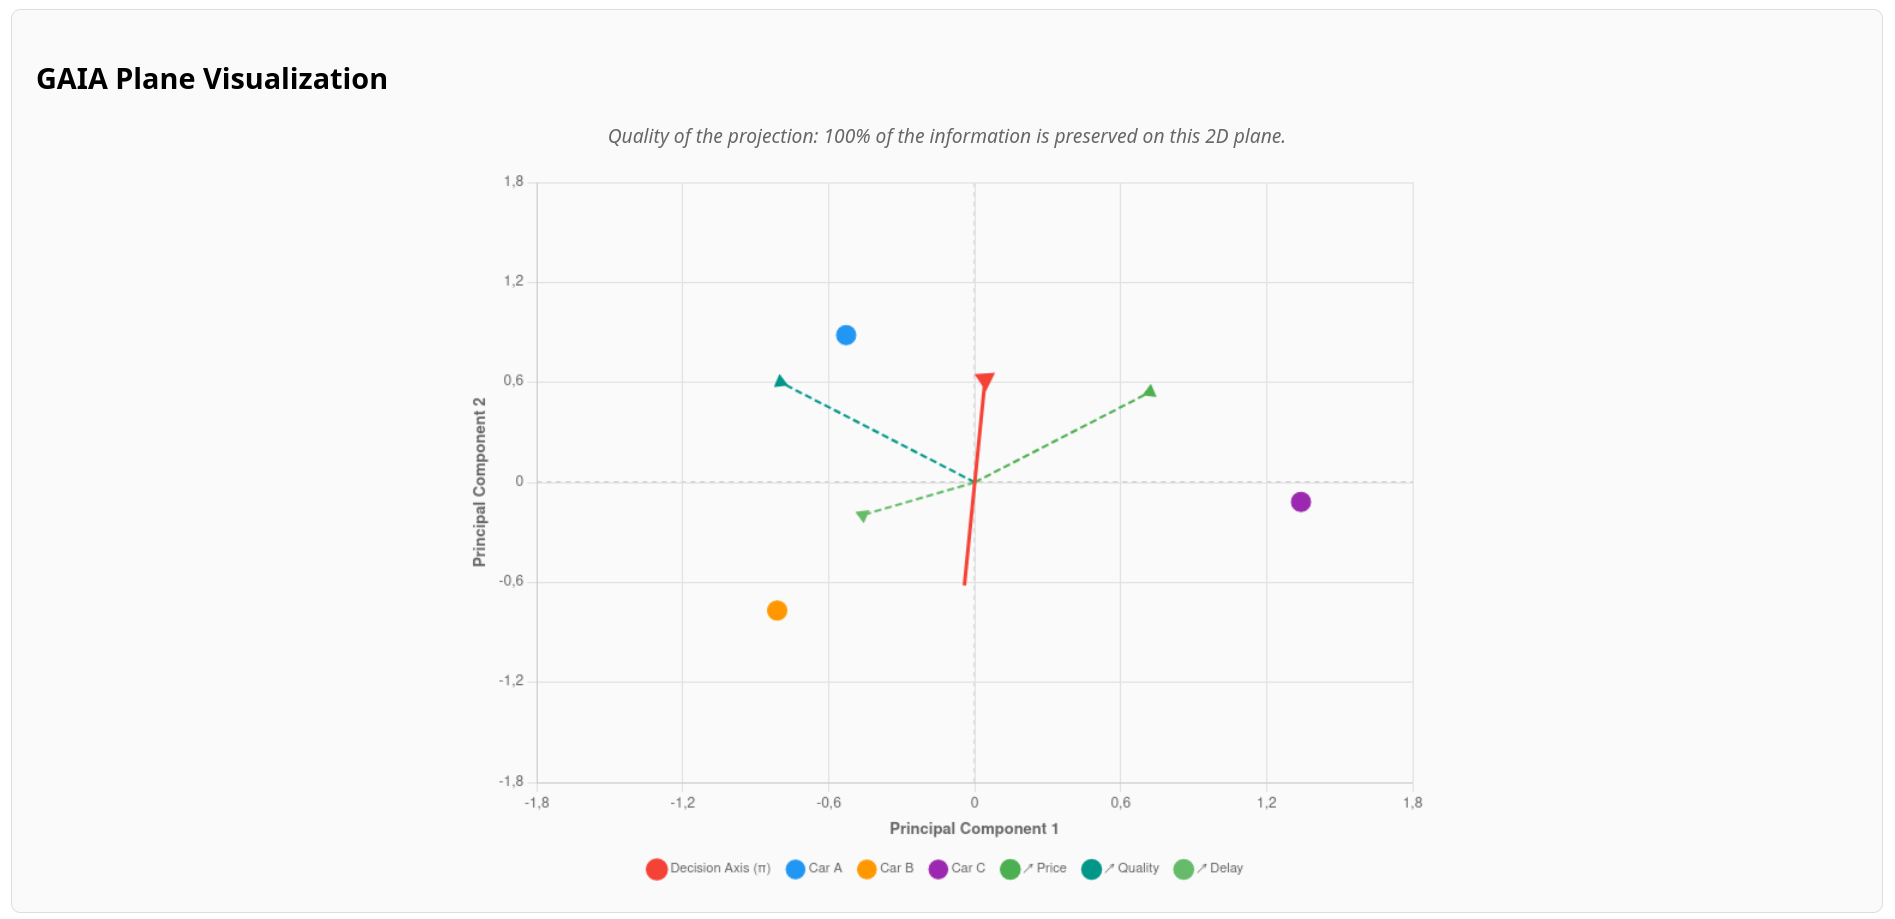
\includegraphics[width=0.85\textwidth]{./res/application_picture/Gaia_Plane.png}
  \caption{GAIA Plane: 2D projection of alternatives (points) and criteria (vectors). The red decision axis $\pi$ points toward the best compromise.}
  \label{fig:gaia_plane}
\end{figure}

\section{Performance Evaluation}
To ensure the application meets enterprise standards, two specific benchmarks were conducted: an algorithmic benchmark of the mathematical engine, and a load test of the web API.

\subsection{Algorithmic Performance}
The time complexity of the PROMETHEE algorithm is theoretically $\mathcal{O}(N^2 \times C)$, where $N$ is the number of alternatives and $C$ the number of criteria. To verify this, a Java benchmark was developed to measure the execution time of the \texttt{PrometheeEngine} class with varying numbers of alternatives and 10 criteria.

\begin{table}[H]
\caption{Algorithmic Benchmark: Execution Time vs. Number of Alternatives}
\label{tab:benchmark_algo}
\centering
\begin{tabular}{lcc}
\toprule
\textbf{Alternatives} & \textbf{Criteria} & \textbf{Execution Time (ms)} \\
\midrule
10 & 10 & 0.03 \\
50 & 10 & 0.81 \\
100 & 10 & 3.03 \\
500 & 10 & 83.31 \\
1000 & 10 & 331.81 \\
2000 & 10 & 1499.32 \\
5000 & 10 & 13778.37 \\
\bottomrule
\end{tabular}
\end{table}

The results in Table \ref{tab:benchmark_algo} clearly demonstrate the quadratic scaling. Calculating a matrix of 1000 alternatives takes approximately 330 milliseconds, which is highly efficient for real-time web interactions.

\subsection{Web Server Load Testing}
To evaluate the robustness of the Tomcat Server and the MVC architecture, a stress test was performed using Apache Bench (\texttt{ab}). The test simulated 100 concurrent users sending a total of 1000 calculation requests to the \texttt{/calculate} endpoint with a JSON payload representing a standard decision matrix.

The server successfully processed all requests with zero failures. The application achieved a throughput of \textbf{2143.30 requests per second}, with a mean processing time of \textbf{46.65 milliseconds} per request. The 99th percentile response time was 144 milliseconds, proving that the stateless architecture and JSON serialization layer (Jackson) are highly efficient and reliable under concurrent load.

\section{Analysis: Positives and Limitations}
\textbf{Positives:} The application provides a highly responsive experience through real-time AJAX recalculations. The backend follows SOLID principles and utilizes the DTO pattern for API communication. The application also supports JSON import/export, enabling users to share and reload decision matrices across sessions.

\textbf{Limitations and Future Alternatives:} One observed limitation is that the current frontend architecture does not provide visual feedback when weights do not sum to exactly 1.0 due to floating-point precision issues (e.g., 0.1 + 0.2 + 0.7 = 0.9999... in JavaScript). A rounding mechanism was implemented as a workaround, but a more robust solution would involve server-side weight normalization using arbitrary-precision data types, such as Java's \texttt{BigDecimal}, to completely eliminate floating-point inaccuracies.

Furthermore, adding multi-user authentication would transform the tool into a collaborative platform supporting multiple Decision Makers simultaneously.

\subsection{Theoretical Limitations of PROMETHEE} Beyond implementation choices, the PROMETHEE method itself presents known theoretical limitations. The \textbf{rank reversal} phenomenon can occur when adding or removing an alternative from the set, potentially altering the relative ranking of unrelated alternatives~\cite{mareschal2013}. Additionally, the choice of preference function parameters ($p$, $q$, $s$) remains subjective and can significantly influence the final ranking, requiring careful sensitivity analysis by the Decision Analyst.

%------------------------------------------------------------
\chapter{Conclusions}
%------------------------------------------------------------

\section{Synopsis of Work}
This project delivered a fully functional, containerized web application implementing the PROMETHEE I and II multi-criteria decision analysis methods. The platform provides a dynamic interface for defining complex decision problems, evaluating alternatives through six distinct preference functions, visualizing trade-offs via a custom-built GAIA plane, and persistently storing results in a relational PostgreSQL database. The entire stack is containerized with Docker, ensuring reproducible deployment. The backend follows SOLID principles through a strict MVC architecture with a dedicated Service layer and DAO pattern.

\section{Suggestions for Improvement}
Future iterations should focus on three axes: 
(1) modernizing the frontend architecture for better state management; 
(2) implementing user authentication for multi-user support; and
(3) adding server-side weight normalization to eliminate floating-point precision issues.

\section{Personal Impressions}
Working with Jakarta EE Servlets deepened my understanding of the HTTP request-response lifecycle and stateless API design. Implementing the six preference functions required carefully translating mathematical specifications into robust, tested Java code --- a level of rigor I had not previously exercised. Designing the Docker Compose orchestration also introduced me to professional deployment practices. The Erasmus+ context further challenged me to communicate all technical concepts in English daily, which significantly improved my professional fluency and adaptability in an international environment.

\section{Use of Artificial Intelligence Tools}
In the spirit of academic transparency, I acknowledge the use of Artificial Intelligence (AI) assistants during the development of this project and the drafting of this report. AI tools were primarily utilized as an advanced search engine, for debugging complex code issues, and for refining the professional English phrasing of this technical documentation. 

I estimate that approximately \textbf{40\%} of the code (mainly structural boilerplate, CSS styling, and LaTeX formatting) and \textbf{50\%} of the linguistic text revisions were assisted by AI. However, the core architectural decisions, the integration of the PROMETHEE mathematical logic, and the overall system design remain my original intellectual work and understanding.

%============================================================
%  Glossary
%============================================================
\chapter*{Glossary}
\addcontentsline{toc}{chapter}{Glossary}
\begin{description}
    \item[DM (Decision Maker)] The person who needs to choose between alternatives and expresses preferences.
    \item[DA (Decision Analyst)] The expert guiding the DM through the application of an MCDA method.
    \item[MCDA] Multi-Criteria Decision Analysis, a sub-discipline of operations research that evaluates multiple conflicting criteria in decision making.
    \item[GAIA Plane] Geometrical Analysis for Interactive Aid --- a 2D visualization obtained by PCA on the unicriterion flow matrix.
    \item[PCA] Principal Component Analysis --- a dimensionality reduction technique that projects high-dimensional data onto a lower-dimensional plane while preserving maximum variance.
    \item[Alternative] A potential choice or option evaluated in the decision-making process.
    \item[Criterion] An attribute or characteristic used to evaluate and compare alternatives.
    \item[Preference Function] A mathematical function used to transform the difference between two evaluations into a preference degree between 0 and 1.
    \item[Indifference Threshold ($q$)] The maximum difference between two evaluations that is considered negligible.
    \item[Preference Threshold ($p$)] The minimum difference between two evaluations that results in a strict preference.
    \item[Outranking] A relation indicating that one alternative is at least as good as another.
    \item[Net Flow] The final score combining positive and negative flows in PROMETHEE II.
    \item[DTO (Data Transfer Object)] An object used to encapsulate data and send it from one subsystem of an application to another.
\end{description}
%============================================================
%  REFERENCES
%============================================================
\cleardoublepage
\addcontentsline{toc}{chapter}{References}

\begin{thebibliography}{99}

\bibitem{brans1985}
J.P. Brans and P. Vincke, ``A Preference Ranking Organisation Method: (The PROMETHEE Method for Multiple Criteria Decision-Making),'' \textit{Management Science}, vol. 31, no. 6, pp. 647--656, 1985.

\bibitem{belton2002}
V. Belton and T. Stewart, \textit{Multiple Criteria Decision Analysis: An Integrated Approach}. Boston: Kluwer Academic Publishers, 2002.

\bibitem{mareschal2013}
B. Mareschal, ``The PROMETHEE Methods,'' in \textit{Multiple Criteria Decision Analysis: State of the Art Surveys}, J. Figueira, S. Greco, and M. Ehrgott, Eds. New York: Springer, 2013.

\bibitem{jakartaee}
Eclipse Foundation, ``Jakarta EE 10 Documentation,'' [Online]. Available: \url{https://jakarta.ee/specifications/platform/10/}.

\bibitem{jackson}
FasterXML, ``Jackson Data Processor Documentation,'' [Online]. Available: \url{https://github.com/FasterXML/jackson-docs}.

\bibitem{TomcatDoc}
Apache Software Foundation, ``Apache Tomcat 10.1 Documentation,'' [Online]. Available: \url{https://tomcat.apache.org/tomcat-10.1-doc/}.

\bibitem{PostgreSQLDoc}
PostgreSQL Global Development Group, ``PostgreSQL 16 Documentation,'' [Online]. Available: \url{https://www.postgresql.org/docs/16/index.html}.

\bibitem{DockerDoc}
Docker Inc., ``Docker Documentation,'' [Online]. Available: \url{https://docs.docker.com/}.

\end{thebibliography}

\end{document}
